\documentclass[sigconf]{acmart}

\usepackage{booktabs} % For formal tables

%\usepackage[ruled]{algorithm2e} % For algorithms
%\renewcommand{\algorithmcfname}{ALGORITHM}
%\SetAlFnt{\small}
%\SetAlCapFnt{\small}
%\SetAlCapNameFnt{\small}
%\SetAlCapHSkip{0pt}
%\IncMargin{-\parindent}

%\IEEEoverridecommandlockouts

\usepackage{colortbl}

\newcommand{\dkcmt}[1]{{\color{red} [{#1}]}}
\newcommand{\rmcmt}[1]{{\color{magenta} [{#1}]}}
\newcommand{\sjcmt}[1]{{\color{blue} [{#1}]}}
\newcommand{\tmcmt}[1]{{\color{orange} [{#1}]}}

\usepackage{tikz}
\usetikzlibrary{shapes,arrows,positioning,decorations.markings,chains,fit,shapes.multipart}
\usepackage{import}
\usepackage{times}
\usepackage{graphicx}
\usepackage{amsfonts}
\usepackage{amssymb}
\usepackage{amsmath}
\usepackage{mathptm}
\usepackage{rotating}
\usepackage{color}
\usepackage{listings}
\usepackage{verbatim}
\usepackage{comment}
\usepackage{alltt}
%\usepackage{subfigure}
\usepackage{mdwlist}
\usepackage{multirow}
\usepackage[algo2e,linesnumbered,ruled,lined]{algorithm2e}
\usepackage{url}
\makeatother

\newcommand{\tool}[1]{\textsc{#1}\xspace}
\newcommand{\symex}{\tool{path-symex}}
\newcommand{\ebmc}{\tool{ebmc}}
\newcommand{\hector}{\tool{hector}}
\newcommand{\slec}{\tool{slec}}
\newcommand{\symexv}{\tool{path-symex 5.0}}
\newcommand{\cbmcv}{\tool{cbmc}}
\newcommand{\cbmcver}{\tool{cbmc 5.2}}
\newcommand{\ebmcv}{\tool{ebmc 4.2}}
\newcommand{\hwcbmcv}{\tool{hw-cbmc}}
\newcommand{\hwcbmcver}{\tool{hw-cbmc 5.0}}
\newcommand{\acdcl}{\tool{acdcl}}
\newcommand{\summarizer}{\tool{summarizer 1.0}}
\newcommand{\abc}{\tool{ABC}}
\newcommand{\yosys}{\tool{Yosys 0.5}}
\newcommand{\verifoxver}{\tool{VerifOx 0.1}}
\newcommand{\verifox}{\tool{VerifOx}}
\newcommand{\iimc}{\tool{iimc}}
\newcommand{\klee}{\tool{klee}}
\newcommand{\symbiotic}{\tool{symbiotic}}
\newcommand{\kleever}{\tool{klee 1.0.0}}
\newcommand{\symbioticver}{\tool{symbiotic 3.0.1}}

\newcommand{\Omit}[1]{}
\newcommand{\scs}[1]{\scriptsize{#1}}

%%% Standard text acronyms

\newcommand{\para}[1]{
  \subsubsection*{#1}}
 
%\noindent
%\textbf{#1~}}

\newcommand{\cnf}{\textsc{cnf}\xspace}
\newcommand{\sat}{\textsc{sat}\xspace}
\newcommand{\smt}{\textsc{smt}\xspace}
\newcommand{\dpll}{\textsc{dpll}\xspace}
\newcommand{\fpdpll}{\textsc{fdpll}\xspace}
\newcommand{\cfg}{\textsc{cfg}\xspace}
\newcommand{\cfgs}{\textsc{cfg}s\xspace}
\newcommand{\acfg}{\textsc{acfg}\xspace}
\newcommand{\smpp}{\textsc{smpp}\xspace}
\newcommand{\cegar}{\textsc{cegar}\xspace}
\newcommand{\cdfl}{\textsc{cdfl}\xspace}
\newcommand{\cdflitv}{\textsc{cdfl}$(\itvdom)$\xspace}
\newcommand{\cdcl}{\textsc{cdcl}\xspace}
\newcommand{\cbmc}{\textsc{cbmc}\xspace}
\newcommand{\bmc}{\textsc{bmc}\xspace}
\newcommand{\cdflalgo}{\textsc{\textsf{cdfl}}\xspace}
\newcommand{\ieeefp}{\textsc{\textsf{IEEE 754}}\xspace}


%%%%%%%%%%%%%%%%%%%%%%%%%%%%%%% 
%%% Mathematical Symbols %%%
%%%%%%%%%%%%%%%%%%%%%%%%%%%%%%% 

%%% Sets and functions

\newcommand{\powerset}[1]{\ensuremath{\wp(#1)}}
\newcommand{\set}[1]{\ensuremath{\left\{#1\right\}}}
\newcommand{\setneg}[1]{\overline{#1}}
\newcommand{\setsep}{\ensuremath{~|~}}
%\newcommand{\tuple}[1]{\ensuremath{(#1)}}

\newcommand{\bnf}{\ensuremath{\mathrel{\mathop{::}}=}}
\newcommand{\bnfsep}{~\mid~}

\newcommand{\true}{\mathsf{true}}
\newcommand{\false}{\mathsf{false}}

%%% Lattices
\newcommand{\sle}{\ensuremath{\sqsubseteq}}
\newcommand{\sles}{\ensuremath{\sqsubset}}
\newcommand{\sge}{\ensuremath{\sqsupseteq}}
\newcommand{\sges}{\ensuremath{\sqsupset}}
\newcommand{\join}{\ensuremath{\sqcup}}
\newcommand{\bigjoin}{\ensuremath{\bigsqcup}}
\newcommand{\meet}{\ensuremath{\sqcap}}
\newcommand{\bigmeet}{\ensuremath{\bigsqcap}}


%%% Program model

\newcommand{\vars}{\mathit{Var}}
\newcommand{\cvars}{\mathit{CVar}}
\newcommand{\vals}{\mathit{Val}}
\newcommand{\exps}{\mathit{Exp}}
\newcommand{\expr}{\mathit{exp}}
\newcommand{\bexps}{\mathit{B\!Exp}}
\newcommand{\envs}{\mathit{Env}}
\newcommand{\env}{\varepsilon}
\newcommand{\aenv}{\hat{\varepsilon}}
\newcommand{\assg}{\ensuremath{\mathrel{\mathop:}=}}
\newcommand{\cond}[1]{\ensuremath{[#1]}}
\newcommand{\choice}[1]{\ensuremath{\mathit{choose}\{#1\}}}
\newcommand{\loopstmt}[1]{\ensuremath{\mathit{loop}\{#1\}}}
\newcommand{\nondetstmt}[1]{\ensuremath{\mathit{nondet}\{#1\}}}
\newcommand{\lfp}{\mathsf{lfp}}
\newcommand{\gfp}{\mathsf{gfp}}

\newcommand{\locs}{\mathit{Loc}}
\newcommand{\stmt}{\ensuremath{\mathit{stmt}}}
\newcommand{\err}{\ensuremath{\lightning}}
\newcommand{\init}{\ensuremath{\mathit{init}}}
\newcommand{\reach}{\mathit{Reach}}
\newcommand{\loopfree}{\mathit{Loop-Free}}

\newcommand{\badprog}{\ensuremath{\mathit{Err}}}
\newcommand{\progexec}{\ensuremath{\mathit{Exec}}}
\newcommand{\absbadprog}{\ensuremath{\hat{\mathit{Err}}}}
% \newcommand{\inv}{\ensuremath{\mathit{Inv}}}
\newcommand{\absinv}{\ensuremath{\hat{\mathit{Inv}}}}
\newcommand{\safe}{\ensuremath{\mathit{Safe}}}
\newcommand{\abssafe}{\ensuremath{\hat{\mathit{Safe}}}}

%%% Standard Abstract interpretation 
%%%
\newcommand{\aenvs}{\mathit{A\!Env}}
\newcommand{\post}{\mathit{post}}
\newcommand{\lpost}[1]{\mathit{post}_{#1}}
\newcommand{\abspost}{\mathit{\hat{post}}}
\newcommand{\abslpost}[1]{\mathit{\hat{post}}_{#1}}

\newcommand{\absuawp}{\mathit{\breve{wp}}}


%%% Fixedpoint-DPLL
%%%
\newcommand{\cvals}{\mathit{CVals}}
\newcommand{\avals}{\mathit{AVals}}

\newcommand{\val}{\mathit{v}}
\newcommand{\aval}{\hat{\mathit{v}}}
\newcommand{\sem}[2]{\ensuremath{\llbracket #1 \rrbracket_{#2}}}
\newcommand{\rsem}[3]{\ensuremath{\llbracket #1 \rrbracket_{#2}^{#3}}}
\newcommand{\asem}[2]{\ensuremath{\|#1 \|_{#2}}}

\newcommand{\comps}{\mathit{Comp}}
%%\newcommand{\ccomp}[1]{\tilde{#1}}
\newcommand{\ccomp}[1]{\mathord{\sim}{#1}}
\newcommand{\rest}{R}
\newcommand{\makerest}[1]{\mathit{res}(#1)}
\newcommand{\restrictions}{\mathit{Res}}
\newcommand{\lrestrictions}{\mathit{LRes}}
\newcommand{\restrict}[2]{\ensuremath{#1\mathord{\downharpoonright_{#2}}}}
\newcommand{\implabel}{\mathit{st}}
\newcommand{\gimplabel}{\mathit{stg}}

\newcommand{\decs}{\mathit{Dec}}
\newcommand{\dec}{\mathsf{d}}
\newcommand{\imp}{\mathsf{i}}
\newcommand{\emptystack}{\epsilon}

\newcommand{\lit}{\ell}
\newcommand{\lits}{\mathit{Lit}}
\newcommand{\litseq}{L}
\newcommand{\stackres}[1]{\lfloor #1\rfloor}
\newcommand{\litrest}[1]{\langle#1\rangle}
\newcommand{\litres}{\mathit{lit}}

\newcommand{\solver}[2]{#1 ~\|~ #2}

%%% Pseudocode
\newcommand{\pdeduce}{\mathsf{deduce}}
\newcommand{\pdecide}{\mathsf{decide}}
\newcommand{\pmaximal}{\mathsf{maximal}}
\newcommand{\plearn}{\mathsf{learn}}
\newcommand{\pbacktrack}{\mathsf{backtrack}}
\newcommand{\pfail}{\mathsf{fail}}
\newcommand{\psafe}{\mathsf{safe}}

 \newcommand{\fpfont}[1]{\textbf{\sffamily{#1}}}
 \newcommand{\fpfn}[1]{\sffamily{#1}}
 \SetKwSty{fpfont}
 \SetFuncSty{fpfn}

 \SetKwFunction{Decide}{decide}
 \SetKwFunction{TransProp}{tprop}
 \SetKwFunction{UnitProp}{uprop}
 \SetKwFunction{Refines}{refines}
 \SetKwFunction{Deduce}{deduce}
 \SetKwFunction{IsUnit}{is\_unit}
 \SetKwFunction{Propagate}{propagate}
 \SetKwFunction{Invariant}{invariant}
 \SetKwFunction{Atomic}{atomic}
 \SetKwFunction{Learn}{learn}
 \SetKwFunction{Backtrack}{backtrack}
 \SetKwFunction{Clausegen}{clauseGen}
 \SetKwFunction{Invariantgen}{invariantGen}

 \SetKw{Let}{let}

%%% Generalization
\SetKwFunction{Asserting}{asserting}
\SetKwFunction{Cutheur}{cutheur}
\SetKwFunction{Generalise}{generalise}
\SetKwFunction{Analyse}{analyse}
\SetKwFunction{ClauseGeneralise}{clauseGeneralise}
\SetKwFunction{WpGeneralise}{wpGeneralise}
\SetKw{MyCase}{case}
\SetKwFunction{SetReason}{setReason}
\SetKwFunction{PickAssertingCut}{assertingCut}
\newcommand{\reasons}{\mathit{Reasons}}
\newcommand{\implicationgraph}{\mathit{implicationGraph}}

%%% Operators
\newcommand{\wrt}{w.r.t.\ }
% \newcommand{\inp}{\mathit{input}}
\newcommand{\M}{{\cal M}}
\newcommand{\Tr}{{\mathit{tr}}}
\newcommand{\clip}{{\mathit{clip}}}
\newcommand{\decomp}{{\mathit{decomp}}}
\newcommand{\form}{{\mathit{Form}}}
\newcommand{\clausecompl}{\mathit{clcomp}}
\newcommand{\covers}{{\mathit{covers}}}
\newcommand{\cfgdecomps}{{\cal D}_{\mathit{CFG}}}
\newcommand{\cfgrefine}{{\cal R}_{\mathit{CFG}}}
\newcommand{\literals}{{\cal L}}
\newcommand{\clauses}{{\cal C}}
\newcommand{\proofstate}{\mathit{proof}}
\newcommand{\literaldecomp}[1]{\mathit{lits(}#1\mathit{)}}
\newcommand{\transded}{\mathit{trans}}
\newcommand{\unitded}{\mathit{unit}}

\newcommand{\prog}{P}

\newcommand{\intervals}{\mathit{Itv}}
\renewcommand{\min}{\mathit{min}}
\renewcommand{\max}{\mathit{max}}
\newcommand{\itvdom}{{\mathit{IEnv}}}
\newcommand{\atoms}{\mathit{Atoms}}

\newcommand{\irred}{\mathit{Irred}_\meet}

\newcommand{\implsu}{I_\mathsf{u}}
\newcommand{\implst}{I_\mathsf{t}}

\newcommand{\predec}{\mathit{predec}}
\newcommand{\conflictnode}{\mathit{conflict}}

\newcommand{\dred}[1]{\textcolor{red!60!black}{#1}}
\newcommand{\dgreen}[1]{\textcolor{green!40!black}{#1}}
%Different kind of brackets
\newcommand{\tuple}[1]{\ensuremath{\langle #1 \rangle}}
\newcommand{\inparan}[1]{\left(#1\right)}
\newcommand{\inbraces}[1]{\{#1\right\}}
\newcommand{\insquareb}[1]{\ensuremath{\left[#1\right]}}

\newcommand{\theoref}[1]{Thm.~\ref{The:#1}}
\newcommand{\theorefs}[2]{Thms.~\ref{The:#1} and~\ref{The:#2}}
\newcommand{\theorefsp}[3]{Thms.~\ref{The:#1}, \ref{The:#2}, and~\ref{The:#3}}
\newcommand{\lemref}[1]{Lem.~\ref{Lem:#1}}
\newcommand{\lemrefs}[2]{Lemmas~\ref{Lem:#1} and~\ref{Lem:#2}}
\newcommand{\lemrefsp}[3]{Lemmas~\ref{Lem:#1},~\ref{Lem:#2}, and~\ref{Lem:#3}}
\newcommand{\corref}[1]{Cor.~\ref{Cor:#1}}
\newcommand{\figref}[1]{Fig.~\ref{Fi:#1}}
\newcommand{\figrefs}[2]{Figs.~\ref{Fi:#1} and~\ref{Fi:#2}}
\newcommand{\defref}[1]{Defn.~\ref{De:#1}}
\newcommand{\defrefs}[2]{Defns.~\ref{De:#1} and~\ref{De:#2}}
\newcommand{\sdefref}[1]{Strawman Defn.~\ref{De:#1}}
\newcommand{\lineref}[1]{line~[\ref{Li:#1}]}
\newcommand{\linerefs}[2]{lines~[\ref{Li:#1}] and~[\ref{Li:#2}]}
\newcommand{\linerefsp}[3]{lines~[\ref{Li:#1}], [\ref{Li:#2}], and~[\ref{Li:#3}]}
\newcommand{\linerefspp}[4]{lines~[\ref{Li:#1}], [\ref{Li:#2}], [\ref{Li:#3}], and~[\ref{Li:#4}]}
\newcommand{\lineseqref}[2]{lines~[\ref{Li:#1}]--[\ref{Li:#2}]}
\renewcommand{\eqref}[1]{Eqn.~(\ref{Eq:#1})}
\newcommand{\eqrefs}[2]{Eqns.~(\ref{Eq:#1}) and~(\ref{Eq:#2})}
\newcommand{\eqrefsp}[3]{Eqns.~(\ref{Eq:#1}), (\ref{Eq:#2}), and~(\ref{Eq:#3})}
\newcommand{\eqrefspp}[4]{Eqns.~(\ref{Eq:#1}), (\ref{Eq:#2}), (\ref{Eq:#3}), and~(\ref{Eq:#4})}
\newcommand{\eqrefspOr}[3]{Eqns.~(\ref{Eq:#1}), (\ref{Eq:#2}), or~(\ref{Eq:#3})}
\newcommand{\eqrefsppOr}[4]{Eqns.~(\ref{Eq:#1}), (\ref{Eq:#2}), (\ref{Eq:#3}), or~(\ref{Eq:#4})}
\newcommand{\eqseqref}[2]{Eqns.~(\ref{Eq:#1})--(\ref{Eq:#2})}
\newcommand{\formref}[1]{Formula~(\ref{Eq:#1})}
\newcommand{\formrefs}[2]{Formulas~(\ref{Eq:#1}) and~(\ref{Eq:#2})}
\newcommand{\formrefsw}[2]{Formulas~(\ref{Eq:#1}) with~(\ref{Eq:#2})}
\newcommand{\formrefsp}[3]{Formulas~(\ref{Eq:#1}), (\ref{Eq:#2}), and~(\ref{Eq:#3})}
\newcommand{\formrefspp}[4]{Formulas~(\ref{Eq:#1}), (\ref{Eq:#2}), (\ref{Eq:#3}), and~(\ref{Eq:#4})}
\newcommand{\formrefspOr}[3]{Formulas~(\ref{Eq:#1}), (\ref{Eq:#2}), or~(\ref{Eq:#3})}
\newcommand{\formrefsppOr}[4]{Formulas~(\ref{Eq:#1}), (\ref{Eq:#2}), (\ref{Eq:#3}), or~(\ref{Eq:#4})}
\newcommand{\tableref}[1]{Tab.~\ref{Ta:#1}}
\newcommand{\tablerefs}[2]{Tabs.~\ref{Ta:#1} and~\ref{Ta:#2}}
\newcommand{\sectref}[1]{Section~\ref{Se:#1}}
\newcommand{\sectrefs}[2]{Sections~\ref{Se:#1} and~\ref{Se:#2}}
\newcommand{\sectrefsp}[3]{Sections~\ref{Se:#1}, \ref{Se:#2}, and~\ref{Se:#3}}
\newcommand{\sectseqref}[2]{Sections~\ref{Se:#1}--\ref{Se:#2}}
\newcommand{\appref}[1]{Appendix~\ref{App:#1}}
\newcommand{\apprefs}[2]{Apps.~\ref{App:#1} and~\ref{App:#2}}
\newcommand{\exref}[1]{Ex.~\ref{Exa:#1}}
\newcommand{\exrefs}[2]{Exs.~\ref{Exa:#1} and~\ref{Exa:#2}}
\newcommand{\exrefsp}[3]{Exs.~\ref{Exa:#1}, \ref{Exa:#2}, and~\ref{Exa:#3}}
\newcommand{\exrefspp}[4]{Exs.~\ref{Exa:#1}, \ref{Exa:#2}, \ref{Exa:#3}, and~\ref{Exa:#4}}
\newcommand{\ruleref}[1]{Rule~(\ref{Rule:#1})}
\newcommand{\rulerefs}[2]{Rules~(\ref{Rule:#1}) and~(\ref{Rule:#2})}
\newcommand{\rulerefsp}[3]{Rules~(\ref{Rule:#1}), (\ref{Rule:#2}), and~(\ref{Rule:#3})}
\newcommand{\rulerefspp}[4]{Rules~(\ref{Rule:#1}), (\ref{Rule:#2}), (\ref{Rule:#3}), and~(\ref{Rule:#4})}
\newcommand{\prodref}[1]{Prod.~(\ref{Prod:#1})}
\newcommand{\prodrefs}[2]{Prods.~(\ref{Prod:#1}) and~(\ref{Prod:#2})}
\newcommand{\prodrefsp}[3]{Prods.~(\ref{Prod:#1}), (\ref{Prod:#2}), and~(\ref{Prod:#3})}
\newcommand{\prodrefspp}[4]{Prods.~(\ref{Prod:#1}), (\ref{Prod:#2}), (\ref{Prod:#3}), and~(\ref{Prod:#4})}
\newcommand{\constraintref}[1]{Constraint~(\ref{Eq:#1})}
\newcommand{\constraintrefs}[2]{Constraints~(\ref{Eq:#1}) and~(\ref{Eq:#2})}
\newcommand{\constraintrefsp}[3]{Constraints~(\ref{Eq:#1}), (\ref{Eq:#2}), and~(\ref{Eq:#3})}
\newcommand{\itemref}[1]{item~\ref{It:#1}}
\newcommand{\itemrefs}[2]{items~\ref{It:#1} and~\ref{It:#2}}
\newcommand{\itemrefsp}[3]{items~\ref{It:#1}, \ref{It:#2}, and~\ref{It:#3}}
\newcommand{\itemrefspp}[4]{items~\ref{It:#1}, \ref{It:#2}, \ref{It:#3}, and~\ref{It:#4}}
\newcommand{\itemseqref}[2]{items~[\ref{It:#1}]--[\ref{It:#2}]}
\newcommand{\Itemref}[1]{Item~\ref{It:#1}}
\newcommand{\Itemrefs}[2]{Items~\ref{It:#1} and~\ref{It:#2}}
\newcommand{\Itemrefsp}[3]{Items~\ref{It:#1}, \ref{It:#2}, and~\ref{It:#3}}
\newcommand{\Itemrefspp}[4]{Items~\ref{It:#1}, \ref{It:#2}, \ref{It:#3}, and~\ref{It:#4}}
\newcommand{\Itemseqref}[2]{Items~[\ref{It:#1}]--[\ref{It:#2}]}
\newcommand{\algref}[1]{Alg.~\ref{Alg:#1}}
\newcommand{\algline}[1]{(Line~\ref{#1})}
\newcommand{\algtwolines}[2]{(Line~\ref{#1} and~\ref{#2})}
\newcommand{\alglines}[2]{(Lines~\ref{#1}--\ref{#2})}
\newcommand{\algrefs}[2]{Algs.~\ref{Alg:#1} and~\ref{Alg:#2}}
\newcommand{\algrefsp}[3]{Algs.~\ref{Alg:#1}, \ref{Alg:#2}, and~\ref{Alg:#3}}
\newcommand{\algrefspp}[4]{Algs.~\ref{Alg:#1}, \ref{Alg:#2}, \ref{Alg:#3}, and~\ref{Alg:#4}}
\newcommand{\assumptionref}[1]{Assumption~(\ref{Assumption:#1})}
\newcommand{\assumptionrefs}[2]{Assumptions~(\ref{Assumption:#1}) and~(\ref{Assumption:#2})}
\newcommand{\footnoteref}[1]{footnote~\ref{Footnote:#1}}
\newcommand{\footnoterefs}[2]{footnote~\ref{Footnote:#1} and~\ref{Footnote:#2}}



\title{Mining Scenario/Transaction Pairs HW/SW Co-verification Using Symbolic Execution}
%===============================================================================
\begin{abstract}
%===============================================================================
%
Time-to-market pressure requires early development of firmware and other
drivers for circuitry well before RTL is finished.  A key risk is divergence
of the hardware RTL from the behavior expected by the software.  Formal
methods can deliver proof that the RTL and the firmware match, but are
difficult to scale up.  We propose to identify partitions of the firmware and
the RTL that follow transaction boundaries by means of path-based symbolic
simulation with custom path-pruning.  We have implemented this approach in
our tool \verifox.  We have experimentally compared \verifox with a
conventional approach, which constructs a single monolithic SAT/SMT
instance, and observe speedups of an order of magnitude over conventional 
approach for proving safety properties as well as detecting firmware/hardware bugs.
%
\end{abstract}            

\begin{document}
\settopmatter{printacmref=false} % Removes citation information below abstract
\renewcommand\footnotetextcopyrightpermission[1]{} % removes footnote with conference information in first column
\pagestyle{plain} % removes running headers
\setcopyright{none}

\maketitle

%
%===============================================================================
\section{Introduction}
%===============================================================================
Hardware/software co-verification is broadly performed at two different
phases in the design cycle: pre-RTL and post-RTL.  In the pre-RTL phase,
engineers write high-level software (SW) models for Intellectual Property (IP), 
which are commonly known as {\em Transaction Level Model}s
(TLM)~\cite{codes14}.  TLMs are typically implemented using the SystemC TLM
library~\cite{tlm} or as plain C programs.  The goal of a TLM is to capture
enough functionality of the hardware (HW) such that it is possible to execute the
SW (drivers/firmware) against it.  Consequently, the TLMs are
incomplete, as they are designed to contain only those behaviors that are
observable by the SW (the drivers or firmware).  In particular, TLMs
are often not cycle-accurate.  These models are used to verify high-level
functionality of the system well before the RTL is
available~\cite{codes14,codes15}. Co-verification of the TLM and the
SW is typically performed by means of testing.

In the post-RTL phase, when the RTL design is available, hardware/software
co-verification becomes more complex.  Unlike the TLM, which only captures
limited design functionality, the RTL implements cycle-accurate behavior
of the final HW, and addresses concerns related to power, area and
timing.  Verification is mandatory to assert that the driver or firmware (FW) 
is executed correctly together with the RTL.  However, the verification of
FW given in C/C++ together with the RTL given in a hardware
description language (HDL) such as Verilog/VHDL is a challenging task due to
the timing and semantic mismatch between the two models -- for example,
FW running on a processor could be much faster than the HW
model it interacts with.  The effectiveness of testing is
thus severely limited in post-RTL co-verification.

Common practice in industry for system-level co-verification is to 
either use emulators/accelerators or Instruction Set Simulators (ISS). 
However, no rigorous formal verification effort is
performed at the post-RTL phase to ensure the validity of the
FW-HW interactions~\cite{vlsid13}.  With this aim in mind, the
primary contribution of this paper is to develop an automated and scalable
hardware/software co-verification methodology that detects FW-HW bugs in the 
presence of an RTL implementation.  

Note that whenever we refer to ``hardware'' from this point onwards, we mean
an RTL implementation and not a TLM.  A firmware services the requests from
the application software layer or its interacting hardware components. 
Similarly, the hardware services the requests from the firmware or the
physical environment.  Thus, the firmware and its interacting hardware
components can be seen as a set of services.  In this paper, we call a
hardware RTL service a {\em Hardware Transaction} $(\mathcal{HT})$.  Closest
to our notion of $\mathcal{HT}$ is the micro-architecture-level transaction
by Mahajan et al.~\cite{mcbmq}.  We call a FW service a {\em Firmware
Transaction} ($\mathcal{FT}$).  $\mathcal{FT}$ is an untimed finite-state
machine that is manifested as control-flow paths in the FW, similar to
transactions in TLM~\cite{codes14}.  A~{\em scenario} $(\mathcal{S})$ in a
co-verification environment typically configures the hardware in a way that
restricts the interaction between $\mathcal{FT}$ and $\mathcal{HT}$.  In
other words, given a $\mathcal{S}$, the firmware only exercises a fragment
of the HW state-space.  This renders many interactions between
$\mathcal{HT}$ and $\mathcal{FT}$ infeasible.  A {\em Scenario/Transaction}
pair is a set of valid interactions between $\mathcal{HT}$ and
$\mathcal{FT}$ for a particular~$\mathcal{S}$.  Thus, it is necessary to
automatically mine Scenario/Transaction pairs to scale HW/SW co-verification
to SoC level designs.  A conventional, monolithic approach, e.g., an
approach based on BMC~\cite{CKY03}, cannot exploit this infeasibility.  The
key idea in this paper is to use path-based symbolic execution to
automatically infer such Scenario/Transaction pairs and check their validity
using backend solvers.

\Omit{
A system is comprised of a set of concurrent FW and HW transactions which
interleaves asynchronously. It is well recognized that concurrency is at
the heart of co-verification. The number of interleavings between the FW
and HW threads can be large, which can become a bottleneck in the
verification process. }

The concurrency between the HW and SW components is a key challenge in
co-verification.  In this paper, we exploit specific interaction patterns
between the FW and HW to reduce the number of interleavings.  We observe
that this interaction pattern follows a producer-consumer relationship --
the master module (producer) solely updates the shared registers which are
consumed by the slave (consumer).  This key observation allows us to
sequentialize a concurrent FW-HW model following specific interaction
patterns.

Generating a unified FW-HW model for co-verification is a well-known 
technique. Notably, Kurshan et al.~modeled HW and 
SW using finite state machines~\cite{fmsd02}, Monniaux in~\cite{emsoft07} modeled
HW and SW as C programs which are formally pushdown systems (PDS), 
Li et al.~in~\cite{fase10} used Buchi Automata to abstractly
model a hardware and PDS to abstractly model a software to generate a unified SW-HW model, 
called Buchi Pushdown System ({\em BPDS}). In this paper, we propose an 
orthogonal approach for co-verification.  
The HW RTL model in Verilog is automatically synthesized to a 
word-level cycle-accurate representation, called, 
{\em software netlist} $(\mathcal{SN})$, in ANSI-C~\cite{mtk2016}. 
The FW model is then instrumented with the call to the 
top level procedure of $\mathcal{SN}$ following specific FW-HW interaction 
patterns. Note that the top level procedure in $\mathcal{SN}$
is the same as the top level module in HW, since the 
synthesis step from RTL to $\mathcal{SN}$ preserves the 
RTL module hierarchy. This results in a unified single-threaded software model, 
that contains both FW and $\mathcal{SN}$ 
(synthesized hardware RTL). We call this 
unified FW-HW model, a {\em program netlist} (${\mathcal{PN}}$). 
This representation enables us to apply
broad range of verification techniques which have 
been less commonly explored in formal hardware/software 
co-verification based on netlists. In particular, we 
apply path-based symbolic execution and bounded model checking (BMC). 
In this paper, we present a path-based symbolic execution tool, 
\verifox, to uncover FW-HW design bugs in ${\mathcal{PN}}$. 
We compare our tool with the state-of-the-art BMC based 
co-verification tool, \hwcbmcv. Our experimental results show 
that path-based symbolic execution is order of magnitude 
faster than the BMC based approaches. 

%===============================================================================
%\subsection{Contributions}
%===============================================================================
In this paper, we make the following contributions:
\begin{enumerate}
\item {\em Co-verification using Symbolic Execution:} 
In this paper, we introduce a notion of {\em transaction} 
in HW RTL and FW models. We present a unified FW-HW model, 
called {\em Program Netlist}, in C, for the co-verification task. 
To this end, we present a path-based symbolic execution algorithm that is 
able to automatically find scenario/transaction pairs from a 
program netlist and check their validity. 
To the best of our knowledge, this is the first attempt to 
perform path-based symbolic execution of 
C (FW) and Verilog RTL (HW) models by synthesizing 
them to a unified program netlist model. 

\item {\em {\verifox} -- A tool for HW/SW co-verification:} We address the
co-verification problem at post-RTL phase and present a tool, \verifox, for
bounded HW/SW co-verification of IP level and SoC level design.  \verifox
supports IEEE 1364-2005 System Verilog standards and the C89, C99 standards. 
\verifox also supports SAT and SMT backends for constraint solving.  We
distribute the HW/SW co-verification tools, \hwcbmcv and \verifox, along
with hardware benchmarks in Verilog RTL and firmware C models
here~\footnote{https://drive.google.com/folderview?id=0BynC6sd-wTYgWVQ4bXNtRDB5a2c\&usp=sharing}. 
\end{enumerate}

\section{Scenarios and Transaction}
%\section{Preliminaries}
In this section, we start by presenting a running example of FW, followed
by some definitions and notations.\\    
%===============================================================================
\subsection{Running Example}
{\bf Running example: }
%===============================================================================
Figure~\ref{firmware} gives a fragment of a FW model for a Universal 
Asynchronous Transmitter/ Receiver (UART) IP.  The
$wb$ class of functions communicate with the {\em wishbone} bus interface to
set/reset the UART input ports and read/write data through the bus
interface.  The FW implements Linux style inb() and outb() functions which
invokes the $wb$ functions to communicate with the UART.  Due to space
limitation, we could not accommodate all $wb$ functions.  The FW begins by
resetting the UART IP which is followed by a $wb\_idle()$ function.  The 
FW then configures the UART in {\em loopback} mode using $outb$ function calls. 
Inside the loop, the firmware checks for a {\em transmitter} or {\em
receiver} interrupt by reading the Interrupt Status register $(UART\_IS)$. 
Depending on the type of interrupt, the firmware either receives a data packet 
or sends a data packet over the serial output. We verify that the transmitted 
data is the same as the received data in the {\em loopback} mode using an 
assertion in the firmware model. Note that $set\_inputs()$ and
$next\_timeframe()$ functions, used in $wb$ functions, are 
primitives in \textsc{HW-CBMC} that direct the tool to set the 
inputs to the HW signals and advance the HW clock, respectively. 

\Omit{
The $set\_inputs()$ and the $next\_timeframe()$ functions are primitives
in \textsc{HW-CBMC} that direct the tool to set the inputs to the HW
signals and advance the HW clock, respectively.  Recall that $\mathcal{SN}$
is the synthesized word-level representation of HW RTL. In the unified
FW-HW model, $\mathcal{PN}$, these primitives are implemented by invoking
the top level module of $\mathcal{SN}$ which is the top module of the UART
RTL IP core.
}

\Omit{ 
In Figure~\ref{firmware}, the firmware executes scenario, $\mathcal{S}$, 
to configure the UART IP in {\em loopback} mode. A property $\psi$ can be as follows: \\
{\em If the content of memory mapped registers (mode configuration and interrupt 
enable) is, $UART\_MC = 0x13$ and $UART\_IE = 0x03$,  then the serial output of 
the transmitter, $UART\_TX$, should not be in high-impedance $(Z)$ state and 
the transmitter buffer must not be EMPTY.}  \\
Note that the antecedent of the property (configuring the UART in 
loopback with interrupt enabled) defines a scenario and the 
consequent defines the condition on the HW transaction. 
In this example, $\mathcal{T}$ \sjcmt{Where did
$\mathcal{T}$ come from?} is a finite-duration service 
through the UART state machine, $(UART\_TX and UART\_RX)$, that 
is spread over multiple clock cycles. 
}

\begin{figure}[t]
\scriptsize
\begin{tabular}{l|l}
\hline
Wishbone Interface & Main Module \\
\hline
\begin{lstlisting}[mathescape=true,language=C]
typedef unsigned char u8;
unsigned char inb 
 (unsigned long port) {
  return wb_read(port);
}
void outb (u8 value, 
 unsigned long port) {
  wb_write(port, value);
}
void wb_reset(void) {
 rst_i = 1;
 set_inputs();
 next_timeframe();
 rst_i = 0;
 stb_i = 0; 
 cyc_i = 0;
}
void wb_idle() {
 set_inputs();
 next_timeframe();
}
void wb_write(_u32 addr, 
     _u8 b) {
 adr_i = addr;
 dat_i = b;
 we_i = 1;
 cyc_i = 1;
 stb_i = 1;
 set_inputs();
 next_timeframe();
 we_i = 0;
 cyc_i = 0;
 stb_i = 0;
}
\end{lstlisting}
&
\begin{lstlisting}[mathescape=true,language=C]
int main() {
wb_reset();
wb_idle();
// Configure the uart
outb (0x13, UART_MC);  
outb (0x80, UART_CM3);
outb (0x00, UART_CM2);
outb (0x00, UART_CM1);
outb (0x00, UART_CR);  
outb (0x03, UART_IE); 
char tx_b[] = "Hello world";
_u8 status = 0;
char rx_b[100];
int i=0,c=0,d=0;
// data transfer in loopback
for (i=0; i<1990; i++){
if (irq_o){
 status=inb(UART_IS)&0x0c;
 if(istatus==0x0c){
 //it was a tx_empty interrupt
 outb(*(tx_b+c),UART_TR); c++;
 }
 else{ //status==0x04
 //it was an rx_data interrupt
  rx_b[d] = inb(UART_TR); d++;
 }
}else {
 // no interrupt. 
 wb_idle();
 wb_idle();
 }
}
// property
for(i=0; i<=10; i++)
 assert(rx_b[i] == tx_b[i]);
}
\end{lstlisting}
\\
\hline
\end{tabular}
\caption{Firmware model of UART IP}
\label{firmware} 
\end{figure}
%
\textbf{Scenario ($\mathcal{S}$):}
Let $B$ denote a set of all possible behaviors of a system. A scenario is a set of 
constraints $\mathcal{S}$ that restrict the system behaviors
to $B' \subseteq B$. For example, the left hand side of Figure~\ref{fig:st}. 
gives an example scenario for the UART FW shown in Figure~\ref{firmware}. 
Here, $\mathcal{S}$ configure the UART IP in {\em loopback} mode with 
interrupt enabled.

\Omit{ 
\textbf{Use case:}
A {\em Use case} is a set of scenarios that satisfy 
a particular goal. A use case completes successfully 
when that goal is satisfied. A complete set of use cases 
defines all the behaviors required of the system. For example, 
a use case in case of UART IP may be to transmit 
the data through the serial port. A scenario is an 
instance of a use case. 
}
%
\begin{figure}[t]
\scalebox{.55}{\import{figures/}{st.pspdftex}}
\caption{Scenario and Firmware Transaction
\label{fig:st}}
\end{figure}

\textbf{Firmware Transaction ($\mathcal{FT}$):} 
A Firmware Transaction ($\mathcal{FT}$) is an untimed state machine 
with a start state and an end state, which is similar to the notion of 
transactions in TLM~\cite{codes14}. 
Each transition in $\mathcal{FT}$ is guarded with a quantifier free predicates
over FW variables and HW signals.
If the guard evaluates to $TRUE$, it may perform some action, which may be 
read/write data. If the guard is not specified, it is assumed to be $TRUE$.
$\mathcal{FT}$ is often manifested as control-flow paths in the firmware. 
The right hand side of Figure~\ref{fig:st} gives a 
$\mathcal{FT}$ for the UART firmware code shown in Figure~\ref{firmware}. 
It has a start state and an end state. $\mathcal{FT}$ is triggered from 
UART output signal, $irq_o$. An execution of $\mathcal{FT}$, also called a 
FW transaction instance, takes a simple path from start state to end state. 
The path taken by an execution is determined by the state of 
the FW variables or its interacting HW signals. Repeated execution of 
$\mathcal{FT}$ can happen only in a sequential manner.  
 
\textbf{Hardware Transaction ($\mathcal{HT}$):} 
Let us consider a HW RTL design with \textit{input} $\{I\}$, 
\textit{output} $\{O\}$, \textit{wires} $\{Wire\}$ and a set of 
state elements such as \textit{Registers} $\{Reg\}$, \textit{Memory}
$\{Mem\}$ ($Mem$ is a sequence of registers). Here, 
$\{I\} \subseteq \{Wire\}$, and $\{O\} \subseteq \{Reg\} \cup \{Wire\}$.
All state elements are fixed-width unsigned integers. 

Let $\mathcal{G}$ be the set of quantifier free boolean predicates over 
state elements, $\{Reg\}$, $\{Mem\}$, $\{Wire\}$.  
A {\em transaction step}, $\varphi$, is defined by 2 tuple,
$\varphi \equiv \langle \Gamma_{\varphi}, \Delta_{\varphi} \rangle$, where 
$\Gamma_{\varphi} \equiv \{\alpha_1, \alpha_2, \ldots \alpha_{m}\}$
is a set of concurrent state updates to $\{Reg\}$, $\{Mem\}$, $\{Wire\}$ 
and $\Delta_{\varphi} \equiv \{\beta_1, \beta_2, \ldots \beta_{n}\} \subseteq
\mathcal{G}$.

A {\em Hardware Transaction} $(\mathcal{HT}) = (V, \Sigma, \rightarrow, init,
comp)$ is a labelled transition system, where $V$ is a set of transaction steps
$\varphi$ with a unique source vertex, $init \in V$, and a unique sink vertex, 
$comp \in V$, $\Sigma$ is a set of labels such that $\Sigma \subseteq 2^{G}$ and  
$\rightarrow \subseteq V \times \Sigma \times V$ is a set of labelled
transitions.

Each execution of $\mathcal{HT}$ is a non-empty 
sequence of transaction steps where each transaction step 
happens in a single clock. The first step is called {\em initiation event}
(\textit{init}). Assuming the duration of $\mathcal{HT}$ is finite, 
there must exist some distinguishable last completion event (\textit{comp}). 
%Operationally, an execution of $\mathcal{HT}$ begins at \textit{init}. 
After a transaction step $\varphi$ is executed, the set of concurrent state
update $\Gamma_{\varphi}$ is carried out and the value of boolean predicates
in $\Delta_{\varphi}$ is evaluated to determine the next step
$\varphi_{next}$, that is, a predicate $\beta_i \in \Delta_{\varphi}$
enables a transaction step.  This process continues until $\mathcal{HT}$
reaches \textit{comp} state.  Note that $\mathcal{FT}$ can update some state
elements of $\mathcal{HT}$ during its write action, based on which
predicates in $\Delta_{\varphi}$ may be computed. 
Figure~\ref{fig:interleaving2} gives a fragment of $\mathcal{HT}$
corresponding to the top module of UART IP.  Let us consider a possible
execution of $\mathcal{HT}$, $(init \rightarrow t_1 \rightarrow t_4
\rightarrow t_6 \rightarrow comp)$.  At $init$, the FW sets the HW input
signal, $(rst\_i==0)$, based on which the execution follows the edge to
$t_1$.  At $t_1$, the predicate, $cs$, is computed based on HW input
signals, $cyc\_i$, $stb\_i$, $adr\_i$ and $we\_i$.  Assuming that $cs\_i
\&\& we\_i$ holds true, the execution proceeds to step $t_4$ which computes
predicates based on the values in $adr\_i$.  The next step is determined by
the values of predicates, $'UART\_MC, 'UART\_IE, 'UART\_CT$.  Assuming that
$'UART\_MC$ holds true, the execution proceeds to $t_6$.  During the
execution of $t_6$, three parallel state update $(dtr\_no, rts\_no,
loopback)$ and two predicate evaluation ($\beta_1,\beta_2)$ is performed
based on the updates to state elements.  After $t_6$, the execution of
$\mathcal{HT}$ leads to $comp$ and the transaction finishes its execution. 
Note that the dotted edges in $\mathcal{HT}$ denotes that eventually the
execution reaches $comp$.  The update of state elements are shown in
rectangular boxes, whereas the evaluation of boolean predicates are shown
inside the rounded boxes.  The blue arrows point to the state updates or
predicate evaluation at a particular~$\varphi$.

\begin{figure}[t]
\scalebox{.55}{\import{figures/}{fw-hw-interleaving.pspdftex}}
\caption{Some HW Transactions for UART
\label{fig:interleaving2}}
\end{figure}

\textbf{Scenario/Transaction Pairs}
%
A scenario, $\mathcal{S}$, restricts the interaction between $\mathcal{HT}$
and $\mathcal{FT}$.  Similar to service-function based transaction in
TLM~\cite{hvc}, we view $\mathcal{FT}$ and $\mathcal{HT}$ as a set of
service in response to its interacting $\mathcal{HT}$ or $\mathcal{FT}$,
respectively.  A {\em Scenario/Transaction} pair is a set of valid
interactions between $\mathcal{HT}$ and $\mathcal{FT}$ for a
particular~$\mathcal{S}$.  For example, an UART IP contains a {\em
transmitter} and a {\em receiver} module.  Let us assume that a scenario,
$\mathcal{S}$, configure a UART in {\em transmission} mode.  Then the
interaction between $\mathcal{FT}$ and $\mathcal{HT}$ is constrained to
contain only those interactions that are relevant to the {\em transmitter}
module.  By contrast, the interactions with respect to the {\em receiver}
module is irrelevant for $\mathcal{S}$.  However, when $\mathcal{S}$
configures a UART in {\em loopback} mode, then the interaction between
$\mathcal{FT}$ and $\mathcal{HT}$ must contain transactions in {\em
transmitter} as well as {\em receiver} module.

This constrained interactions can be exploited 
to decompose the verification state-space. 
This requires an automatic technique for scenario driven 
partitioning of the FW-HW transactions to generate only 
relevant {\em Scenario/Transaction} pairs. Conventional 
approaches for co-verification construct a unified 
FW-HW model in FSM or BPDS that restrict such decomposition. 
In this paper, we built a unified FW-HW model in C program 
which enable us to automatically generate such {\em scenario/transaction} 
pairs using path-based symbolic execution techniques. The details 
of our technique are explained in the next section.
%
\Omit{
\textbf{Problem Statement}
Given a FW model in C, HW models in Verilog RTL, a property $\psi$ and 
a set of scenarios, the goal is to check whether $\psi$ holds under all 
scenarios in the combined FW-HW model. 
}
%
\section{Proposed Methodology}
Figure~\ref{proposed-flow} describes our overall tool framework. In the
subsequent section, we describe each step in details. 

\begin{figure}[t]
%\centering
\scalebox{.48}{\import{figures/}{work-flow.pspdftex}}
\caption{Proposed HW/SW Co-verification Flow
\label{proposed-flow}}
\end{figure}

%\subsection{Software netlist}
{\bf Software netlist:}
The hardware circuits in Verilog RTL is automatically 
synthesized to a word level C program, called a 
\textit{software netlist}~\cite{mtk2016,mskm2016} using the 
tool {\em v2c}~\cite{mtk2016}. {\em v2c} follows synthesis semantics and not 
simulation semantics. The generated code is cycle-accurate as well as 
bit-precise. {\em v2c} automatically translates concurrent statements 
in Verilog such as procedural blocks and continuous assignments to 
a semantically equivalent C program. 
 
A \textit{software netlist} $\mathcal{SN}$ is defined as follows:
\Omit{
a four-tuple $\langle L, A, l_0, l_e
\rangle$, where $L$ is a finite set of locations, modelling the values of
the program counter in the corresponding sequential code, $l_0 \in L$ is the initial
location, $l_e \in L$ is the error location, and $A \subseteq L \times M
\times L$ is the control flow automaton.  The edges in $A$ are labelled
with a quantifier-free first-order formula over program variables drawn from
the set $M$. These formulas encode an assignment and
take the form $\langle \mathit{In}, \mathit{Out},
\mathit{Seq}, \mathit{Comb}, \mathit{Asgn} \rangle$,
\sjcmt{$M$ is confusing. Is it a set of first order formula
or a set of $Asgn$?}
}
%
\[ 
\begin{array}[t]{@{}lll}
\mathcal{SN} & {:}{:}{=} & \mathit{Modules} \\
\mathit{Modules} & {:}{:}{=} & \epsilon \mid \mathit{moduleName(Var_1,\dots,Var_n)} \{ Asgn \} \;\; Modules \\
\mathit{Asgn} &  {:}{:}{=} & \mathit{CAsgn} \mid \mathit{SAsgn} | moduleName(Var_1,\dots,Var_n)\\
\mathit{CAsgn} & {:}{:}{=} & (V_c := Bv) \mid (V_c := \mathit{Bool}), \quad V_c \in \mathit{Comb} \uplus \mathit{Out} \\
\mathit{SAsgn} & {:}{:}{=} & (V_s := Bv) \mid (V_s := \mathit{Bool}), \quad V_s \in \mathit{Seq} \\
\mathit{Bv} &  {:}{:}{=} & bv_{const} \mid bv_{var} \mid
	\mathit{ITE}(Bool, Bv, Bv) \mid
bv_{op}(bv_1, \ldots, bv_n), \\
& & bv_i \in Bv, \\ 
& & bv_{op} \in \{n-\text{ary operators over bitvectors} \} \\
\mathit{Bool} & {:}{:}{=} & \mathit{true} \mid \mathit{false} \mid \neg{Bool} \mid Bool \land Bool \mid 
Bool \lor Bool \mid \\ 
& & Bv\; relop\; Bv, relop \in \{<,\leq,=,>,\geq\} \\
\end{array}
\]
%
Here, $\mathit{In}$, $\mathit{Out}$, $\mathit{Seq}$, $\mathit{Comb}$
are programs variables that model \emph{input}, \emph{output}, 
\emph{sequential/state-holding} and \emph{combinational/stateless} 
signals in the circuit.  $Asgn$ is a finite set of assignments 
to $Out$, $Seq$ and $Comb$. 

\Omit{
A state transition in HW can be described by a set of register updates,
defined by the next-state function, and assignment of non-deterministic 
values to external inputs. The state transition in the software netlist 
corresponds to updates to the variables in $Seq$ and explicit assignment 
of non-deterministic values to the input variables, $In$.
}

%\subsection{Generating Unified FW-HW model}
\subsection{Analyzing FW/HW interaction Patterns}
%{\bf Analyzing FW/HW interaction pattern: }
The data dependencies between FW and HW is analyzed 
to reduce the number of interleavings between them and 
generate a unified FW-HW model. 
\Omit{
Recall that a HW transaction $(\mathcal{HT})$ is in response to a FW transaction 
$(\mathcal{FT})$. Similarly, $\mathcal{FT}$ is in response to the 
inputs from $\mathcal{HT}$ or operating system or application level software. 
The specific interaction pattern between $\mathcal{FT}$ 
and $\mathcal{HT}$ is exploited to generate a 
unified FW-HW model, $\mathcal{PN}$, in C. 
}
We observe that this interaction pattern follows 
producer-consumer relationship as shown in 
Figure~\ref{fig:interleaving1}. 
\Omit{
In practice, a FW thread 
is mostly independent of the HW thread they interact with~\cite{hvc}.  
Specifically, a FW thread is only responsible for configuring the 
HW transactions by writing to memory mapped registers 
or polling the interrupt status register for data transmission or 
receiving incoming data packets. 
}
We formally define the data dependencies between $\mathcal{FT}$ 
and $\mathcal{HT}$. A communicating pair of executions of 
$\mathcal{FT}$ and $\mathcal{HT}$ is an {\em interaction}, which 
takes place through shared variables (or shared registers)
only.

\Omit{
\textbf{Producer:} 
$\mathcal{FT}$ (or $\mathcal{HT}$) is called a {\em producer} 
if it produces a data ($d$) that is independent of $\mathcal{HT}$ (or $\mathcal{FT}$). 
Thus, the interleavings between $\mathcal{FT}$ and $\mathcal{HT}$ 
can be avoided to compute $d$. 
}

\textbf{Producer-consumer Interaction:}
%
An interaction is said to exhibit {\em producer-consumer}
interaction pattern if 1) the set of variables $V$ written by 
the execution of $\mathcal{FT}$ and and the set of variables 
$V'$ written by the execution of $\mathcal{HT}$ are disjoint 
($V \cap V' = \emptyset$), (2) and the executions 
of $\mathcal{FT}$ and $\mathcal{HT}$ consumes values 
in $V'$ and $V$, respectively.

\Omit{
shared register only FT is writing 
shared register that HT is writing 
and these two sets are disjoint
$\mathcal{FT}$ and $\mathcal{HT}$ is said to exhibit   
{\em producer-consumer} interaction pattern specific 
to data $d$ if $\mathcal{FT}$ produces $d$ and $\mathcal{HT}$ 
consumes $d$. Similarly, when $\mathcal{HT}$
is a producer of $d$ and $\mathcal{FT}$ is a consumer of $d$, 
$\mathcal{HT}$ and $\mathcal{FT}$ is said to exhibit   
{\em producer-consumer} interaction pattern specific to $d$. 
A producer-consumer interaction is defined with respect 
to the data produced. 
}

Figure~\ref{fig:interleaving1} illustrates the FW-HW interaction pattern 
for the UART IP. The FW CFG is shown in the left and the 
HW RTL code snippet is shown in the right. We abuse notations and 
represent $\mathcal{HT}$ in the form of RTL and $\mathcal{FT}$ as CFG
for our illustration purpose. Here, $\mathcal{HT}$ is the producer of interrupt 
status signal, $irq\_o$, which is read by $\mathcal{FT}$ in state $s_1$. 
The signal $irq\_o$ is  triggered when transmitter buffer is 
{\em EMPTY} or receiver buffer is {\em FULL}. 
$\mathcal{HT}$ also produces interrupt status by writing to the 
memory mapped register, $UART\_IS$, which is consumed by 
$\mathcal{FT}$ in state $s_2$.  In another interaction, $\mathcal{HT}$
sends a data-packet to $UART\_TR$ which is consumed by $\mathcal{FT}$ in state $s_7$.
Similarly, $\mathcal{FT}$ is the producer of $data$, $(outb(data,UART\_TR))$, 
in state $s_6$ which is consumed by $\mathcal{HT}$. These interaction patterns 
between $\mathcal{HT}$ and $\mathcal{FT}$ is exploited to generate a 
sequential unified {\em program netlist} model which is defined next.\\ \\
%
\begin{figure}[t]
\scalebox{.55}{\import{figures/}{interleaving.pspdftex}}
\caption{Producer Consumer Interactions Pattern
\label{fig:interleaving1}}
\end{figure}
%
{\bf Unified FW-HW model:}
A {\em program netlist} $\mathcal{PN}$ is a sequential unified
model of FW and HW. $\mathcal{PN}$ is formally defined as follows.
\[ 
\begin{array}[t]{@{}lll}
\mathcal{PN} & {:}{:}{=} & \mathit{Procedure} \\
\mathit{Procedure} & {:}{:}{=} & \mathit{Statement} \mid \mathit{Procedure} \\
\mathit{Statement} & {:}{:}{=} & CStatement \mid \mathit{moduleName(Var_1,\dots,Var_n)} \\
\mathit{CStatement} & {:}{:}{=} & x {:}{=} exp \mid \mathit{ITE}(b, s_1,s_2) \mid \mathit{s_1;s_2} \mid loop\{s\} \\ 
\end{array}
\]
Consider sets of expressions $Exp$ and Boolean expressions $BExp$ 
over variables $Var$ of $\mathcal{PN}$ such that $(exp \in Exp)$ and 
$(b \in BExp)$. A $\mathit{CStatement}$ is an assignment,
conditional, sequential concatenation or a loop.
$\mathit{moduleName(Var_1,\dots,Var_n)}$ invokes the top level 
procedure of the $\mathcal{SN}$. Recall that $\mathcal{SN}$ is a
software netlist representation of HW RTL models.
The interface variables $\{Var\_1,\dots,Var\_n\}$ 
(input, output and inout ports) are declared inside the 
FW to communicate with $\mathcal{SN}$. \\ 
\Omit{
$\mathcal{PN}$ is verification equivalent 
to the concurrent execution of FW and $\mathcal{SN}$.
}
\textbf{Property Driven Slicing of Program Netlist:}
A property-driven slicing is performed on the unified model, $\mathcal{PN}$.  
This step is purely syntactic, meaning that we perform a backward dependency 
analysis starting from the property which only preserve those 
program fragments that are relevant to a given property. The sliced program 
is then passed to the symbolic execution engine for path-based exploration. 
\Omit{
\section{Extracting relevant FW/HW interactions using}
Our unified FW-HW model, $\mathcal{PN}$, is composed of a set of 
FW scenarios, $\{\mathcal{S}\}$, and a set of HW transactions, $\{\mathcal{T}\}$ 
that $\{\mathcal{S}\}$ depends on. However, only a subset of $\{\mathcal{T}\}$ is 
relevant for a particular $\mathcal{S}_i \in \mathcal{S}$. In this section, 
we present a path-based exploration algorithm to automatically infer 
interacting $\mathcal{S}/\mathcal{T}$ pairs from $\mathcal{PN}$. 
}
%=======================================================================================
%\subsection{\verifox: Path-wise Symbolic Execution Tool} 
%=======================================================================================
%\Omit{
%\begin{figure}[tp]
%\centering
%\vspace*{0.3cm}
%\scalebox{.50}{\import{figures/}{work-flow.pspdftex}}
%\caption{Automated Slicing and Trace partitioning\label{fig:desc}}
%\end{figure}
%}
\Omit{
\begin{figure}[t]
\tikzstyle{rblock}=[rounded corners,draw=black]
\tikzstyle{block}=[draw=black]
\begin{tikzpicture}

\node (v2c) [rblock] {\scs{\emph{v2c}}};
\node (snl) [block,below of=v2c] {\scs{Software-netlist}};
\draw[->] (v2c) -- (snl);


\node (HD) [above left=.3cm and .3cm of v2c] {\scs{\parbox{8em}{Hardware Design \\ (in Verilog)}}};
\draw[->] (HD) -- (v2c);

\node (prop) [above right=.3cm and .3cm of v2c] {\scs{\parbox{8em}{Property \\ (in SVA)}}};
\draw[->] (prop) -- (v2c);

\node (cmm) [block,below of=snl] {\scs{\parbox{9em}{Composite Monolithic Model}}};
\draw[->] (snl) -- (cmm);

\node (dcmm) [left=1cm of cmm] {};
\node (fw) [above=.1cm of dcmm  ] {\scs{Firmware}};
\node (as) [below=.1cm of dcmm] {\scs{Assumptions}};
\draw[->] (fw) -- (cmm);
\draw[->] (as) -- (cmm);

\node (pds) [block,below of=cmm] {\scs{\parbox{8em}{Property-driven slicing}}};
\draw[->] (cmm) -- (pds);

\node (tp) [block,below=.8cm of pds] {\scs{Trace partitioning}};
\node (iss) [block,below right=.5cm  and .05cm of tp.east] {\scs{\parbox{6em}{Incremental SAT solving}}};
\node (sat) [rblock,below=1.5cm of tp] {\scs{SAT solver}};
\node (ipp) [block,left=2cm of iss] {\scs{\parbox{6em}{Infeasible path pruning}}};

\draw [<->] (tp) -- (iss);
\draw [<->] (tp) -- (ipp);
\draw [<->] (sat) -- (iss);
\draw [<->] (sat) -- (ipp);

\node (vfbox) [rblock,fit={(tp) (iss) (sat) (ipp)}] {};
\draw[->] (pds) -- (vfbox);

\node (verifox) [right=.2cm of tp] {\scs{{\bf \verifox}}};

\node (safe) [above right=.2cm and .2cm of vfbox.east] {\scs{Verification Successful}};
\node (unsafe) [below right=.2cm and .2cm of vfbox.east] {\scs{\parbox{8em}{Verification Failed (Counterexample)}}};

\draw[->] (vfbox.9) -- (safe);
\draw[->] (vfbox.-12) -- (unsafe);

\end{tikzpicture}
\caption{Automated Slicing and Trace partitioning\label{fig:desc}}
\end{figure}
}

\subsection{Path-based Symbolic Execution}
We have developed a symbolic execution tool, \verifox, 
for FW-HW co-verification of IP level and SoC level designs. 
Given a program netlist model, $\mathcal{PN}$, a scenario, 
$\mathcal{S}$, and a property expressed as $\mathit{assert}(c)$ 
(where $c$ is a condition stated in terms of variables in $\mathcal{PN}$)
as input, \verifox performs path-based exploration of $\mathcal{PN}$ 
to automatically infer {\em scencario/transaction} pairs and check their validity 
using backend solvers. If the condition $c$ does not hold, 
then $\mathcal{PN}$ is said to have violated the property. 


\Omit{
explores only those FW-HW interactions
that are relevant to $\mathcal{S}$. \verifox 

\verifox takes a C program as an input, where 
the properties of interest are specified using 
statements in the code. Here, $c$ is a condition 
stated in terms of program variables that we 
want to hold at the point where the assertion occurs. 
}

\Omit{
 that performs 
path-based exploration of a unified FW-HW model, 
$\mathcal{PN}$ to automatically check the validity of the 
relevant {\em scencario/transaction} pairs of the FW-HW interactions.
}
\Omit {
\verifox performs depth-first exploration 
of program paths with aggressive pruning strategy  
with certain optimizations
that makes it suitable for verifying hardware designs. 
A hardware circuit having its 
behaviour specified in a manner similar to state machine, would usually
be translated into a program that has a large number of control-flow paths with
only tiny fractions of them being feasible. 
}
A typical path-based symbolic execution engine might explore 
a path until it come to an $\mathit{assert}(c)$ statement.
This whole path can then be posed as a query to a SAT solver to see if the 
assertion is violated at that point. If the path is infeasible, the assertion
holds trivially. If a large number of paths are infeasible, symbolic 
execution may waste time exploring them. \verifox employs 
an eager infeasibility check to prune infeasible paths, 
as well as incremental encoding that makes
it easier for the underlying SAT solver. 
\begin{algorithm2e}[t]
\DontPrintSemicolon
\SetKwFunction{symex}{Symex}
%\SetKwFunction{assert}{assert}
\SetKwFunction{put}{put}
\SetKwFunction{get}{get}
\SetKwFunction{print}{print}
\SetKwFunction{return}{return}
%\SetKwFunction{assume}{assume}
%\SetKwFunction{isf}{isFeasible}
\SetKwData{safe}{Safe}
\SetKwData{unsafe}{Unsafe}
\SetKwInOut{Input}{input}
\SetKwInOut{Output}{output}
\SetKw{KwNot}{not}
\begin{small}
\Input{Program Netlist $\mathcal{PN}$ with properties specified with $assert(c)$, scenario specified with $assume(c)$}
\Output{The status (\safe or \unsafe) and a counterexample if \unsafe}
\tcc{The initial state}
$S_0 \leftarrow I(x)$ \nllabel{algline:init}\;
$stmt \leftarrow $ first statement \;
$worklist.put(\tuple{S_0,stmt})$ \;
\While{\KwNot $worklist.empty()$}
{
	$\tuple{S,stmt} \leftarrow worklist.get()$ \;
	\uIf{$stmt$ is an $assume(c)$ \nllabel{algline:assume}}
           {
			$stmt \leftarrow $ statement after $assume(c)$ \;
			\lIf{$isFeasible(S\wedge c)$}{$worklist.put(\tuple{S\wedge c,stmt})$}
              
       		}
	\uElseIf{$stmt$ is a branch with condition $c$ \nllabel{algline:branch}}
	{
		$stmt_f \leftarrow$ first statement after $stmt$ if branch is not taken\;
		$stmt_t \leftarrow$ first statement after $stmt$ if branch is taken \;
		\lIf{$isFeasible(S\wedge c)$}{$worklist.put(\tuple{S\wedge c,stmt_t})$}
		\lIf{$isFeasible(S\wedge \neg c)$}{$worklist.put(\tuple{S\wedge \neg c,stmt_f})$}
		
	}
	\uElseIf{$stmt$ is an $assert(c)$ \nllabel{algline:assert}}
	{
		$stmt \leftarrow $ statement after $assert(c)$ \;
		\If{$isFeasible(S \wedge \neg c)$}{
		\print \unsafe \;
		\return Counterexample}
		\lElse{ $worklist.put(\tuple{S \wedge c,stmt})$}
	}
	\Else
	{
		$S \leftarrow symex(S,stmt)$\; \nllabel{algline:symex}
		$stmt \leftarrow $ the next statement in control flow after $stmt$ \;
		\lIf{$stmt \neq \bot$ \nllabel{algline:nullstmt}} {$worklist.put(\tuple{S,stmt})$} \;
		
	}
	\return \safe \;
}
\end{small}
\caption{Working of \textsc{verifox}\label{Alg:verifox}}
\end{algorithm2e}

\Omit{
, in which every time a branch or an assumption
is encountered, a feasibility check is made to prune away infeasible 
paths as early as possible. }
\vspace{-4mm}
\algref{verifox} shows the overall algorithm of \verifox. States mentioned
in the algorithm are all symbolic states, which are quantifier-free predicates characterizing
a set of program states. 
Symbolic execution starts with an initial symbolic state $I(x)$, is a quantifier-free predicate
over program variables $x$, and the first statement $\mathit{stmt}$ to be executed.  Note that we assume all program variables
have finite bit-width and thus can be represented as bit-vectors.
Every statement acts as a state transformer during the symbolic execution. $\mathit{worklist}$ 
maintains the set of symbolic states, along with the corresponding
$\mathit{stmt}$ that should execute next. Assumptions can be specified in the program 
using $\mathit{assume}(c)$ statements, where $c$ is the condition expressed in terms 
of program variables. Assumptions restrict the search to only those
states for which the condition $c$ holds at the program point where $\mathit{assume}(c)$ is encountered.
For example, suppose $(x!=0)$ characterizes the set of states that has been discovered to be
reachable so far by a verification tool. Here, $x$ is a program variable.
Upon encountering $\mathit{assume}(x>0)$, the 
set of states reachable at the point of assumption is shrunk to only those that
satisfy $(x>0)$. A user can specify assumptions to restrict
the verification to only certain regions of the program's state space.

\verifox performs a feasibility check at an $\mathit{assume}$ statement 
or a branch \algtwolines{algline:assume}{algline:branch} to ensure that
only feasible symbolic states are kept in the $\mathit{worklist}$. This ensures that the
infeasibility is detected as early as possible. 
If an assertion is violated, then a counterexample is detected and \algref{verifox}
terminates \algline{algline:assert}. In all other cases, $\mathit{symex}(S,\mathit{stmt})$ performs
one step of symbolic execution by executing $\mathit{stmt}$ from the symbolic state $S$ \algline{algline:symex}.
If no further statement remains to be executed along the path that is being explored,
then $\mathit{stmt}$ is assigned the value $\bot$. The symbolic state is put in the worklist only 
if there are further statements remaining \algline{algline:nullstmt}.

The feasibility checks shown as $\mathit{isFeasible}$ pose a query to the underlying SAT solver.
Note that \algref{verifox} does not refer to how the methods $\mathit{worklist.put}$ and $\mathit{worklist.get}$
work. In principle, one can use any search heuristic to select which symbolic state to explore 
further from the $\mathit{worklist}$. In the current version \verifox employs a depth first strategy of exploration.

Apart from the eager infeasibility check, another crucial optimization is the
use of incremental SAT solving during the symbolic execution. 
%\verifox can use incremental SAT-solving capabilities in two ways.
During the symbolic execution, only one solver instance is maintained 
while going down
a single path. Thus, when making a feasibility
check from one branch $b_1$ to another branch $b_2$ along a single path, only the program
segment from $b_1$ to $b_2$ is encoded as a constraint and added to the existing solver
instance. 
\Omit{
Internal solver states and the information that it gathers during the search
remains valid as long as all the queries that are posed to the solver in succession are
monotonically stronger. If the solver solves a formula $\phi$, posing $\phi \wedge \psi$ as 
a query to the same solver instance allows one to reuse the solver knowledge that
it has acquired in the previous query, because any assignment that falsifies $\phi$ also
falsifies $\phi \wedge \psi$. Thus the solver need not revisit the assignments that it has already
ruled out.}
This results in speeding up the process of feasibility check of the symbolic state at $b_2$ as
the feasibility check at $b_1$ was $\mathit{true}$. A new
solver instance is used to explore a different path, after the current path is detected as infeasible.

\Omit{
In the full incremental mode, only one solver instance is maintained throughout the whole
 symbolic execution. Let $\phi_{b_1b_2}$ denote the encoding of the path fragment
from $b_1$ to $b_2$. It is added in the solver as $(B_{b_1b_2} \implies \phi_{b_1b_2})$.
Then, $B_{b_1b_2}$ is added as a \textit{blocking variable}, which is also usually known as {\em solver assumption}.\footnote{The SAT community uses the term \textit{assumption variables} or \textit{assumptions}, but we will use the term blocking variable to avoid ambiguity with assumptions in the program.} to enforce constraints specified by $\phi_{b_1b_2}$. Blocking variables are treated specially inside the solvers: unlike regular variables or clauses, the blocking can be removed in subsequent queries without invalidating the solver instance.
When one wants to back-track the symbolic execution, the blocking $B_{b_1b_2}$ is removed 
and a unit clause $\neg B_{b_1b_2}$ is added to the solver, thus effectively removing $\phi_{b_1b_2}$.
}

Eager infeasibility check restrict the search to explore
only those FW/HW interations which are feasible under a
given scenario.
%Eager infeasibility check may save the engine from exploring multiple paths
%that emerge through branches encountered after the first point of infeasibility.
In our experiments, we find this optimization has a large effect on runtimes.
Though \verifox poses many queries to the SAT solver, each query is relatively simple due to
two reasons: the resultant formula encodes only a single path, 
and exploration along a path only needs to encode and solve for the path segment (along with the existing
constraints) from the last point of query.

\Omit{
\rmcmt{
The hardware and firmware run independently of each other. 
The communication between them takes place through interrupts. 
The interrupts are modelled by function calls. 
}
}
%
\section{The Conventional Approach to Co-verification}
%
\begin{figure}[t]
\begin{center}
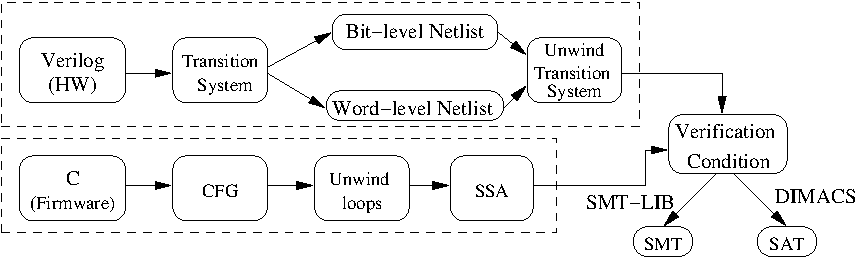
\includegraphics[scale=0.6]{figures/traditional_flow.pdf}
\caption{Conventional HW/SW Co-verification Flow}
\label{fig:conventional}
\end{center}
\end{figure}

Figure~\ref{fig:conventional} illustrates the conventional approach to HW/SW
co-veri\-fi\-cation, as implemented in the state-of-the-art co-verification
tool, \hwcbmcv~\cite{CKY03,vlsid13}.  \hwcbmcv is the only open-source
formal co-verification tool that supports Verilog RTL (System Verilog 2009
standard) and C/C++ firmware.  In contrast to our proposed approach,
\hwcbmcv maintains two separate flows for HW and FW.  The top flow in
Figure~\ref{fig:conventional} uses synthesis to obtain either a bit-level or
a word-level netlist from Verilog RTL.  The bottom flow illustrates the
translation of the C program into static single assignment (SSA) form. 
These two flows meet only at the solver.  Thus, \hwcbmcv generates a
monolithic formula from the C and RTL description, which is then checked
with SAT/SMT solvers.  \hwcbmcv provides specific handshake primitives such
as $next\_timeframe()$ and $set\_inputs()$ to model FW-HW communications.
%
\Omit{
The hardware and firmware run independently of each other. 
The communication between them takes place through these function calls. 
}

%===============================================================================
\section{Experimental Results}
%===============================================================================

We report experimental results for FW-HW co-verification of a UART IP and a
SoC design.  All our experiments were performed on an Intel Xeon 3.07\,GHz
machine with 48\,GB RAM.  We use a state-of-the-art hardware/software
co-verification tool, \hwcbmcv, and compare it against \verifox. 
MiniSAT-2.2.0~\cite{DBLP:conf/sat/EenB05} was used as underlying SAT solver
with \verifoxver, CBMC-5.0~\cite{DBLP:conf/tacas/ClarkeKL04} and
\hwcbmcver~\cite{CK03}.  We also used other path-based symbolic execution
tools, such as, \kleever and \symbioticver for our experiments and presented
a comparison with \verifoxver.  All times reported are in seconds.  The
timeout for all our experiments was set to 2~hours.  The UART IP, SoC
benchmark (Verilog RTL and Firmware in C) and our co-verification
tools,\hwcbmcv and \verifox, are available for
download~\footnote{https://drive.google.com/folderview?id=0BynC6sd-wTYgWVQ4bXNtRDB5a2c\&usp=sharing}.

\Omit{
Even though \verifox supports SMT solvers such as
Z3~\cite{z32008} as backend solvers, the current implementation communicates
with these solvers using files rather than APIs.  Since a new solver
instance is generated for every query, incremental encoding cannot be used. 
Due to this, the runtimes of \verifox with SMT solvers on benchmarks are
significantly higher.  As the current implementation does not support
incremental encoding with SMT solvers, the runtimes would not provide a fair
comparison of \verifox with SMT versus \verifox with SAT solvers. 
Therefore, we are omitting the results obtained using SMT solvers.  

All the benchmarks in
Verilog (excluding commercial ARM IP), software-netlist models in C,
firmware models, our tool \textsc{Verifox} and scripts for running \hwcbmcv,
\cbmc, \textsc{klee} and \textsc{Symbiotic} are available
here~\footnote{https://drive.google.com/file/d/0BynC6sd-wTYgSEU5eEswbnRqWUE/view?usp=sharing}
}

%-------------------------------------------------------------------------------
\subsection{FW-HW co-verification of UART}
%-------------------------------------------------------------------------------

\textbf{\emph{About UART:}} A UART IP core is used for asynchronous
transmission and reception of data which provides serial communication
capabilities with a modem or other external devices.  The UART IP is
compliant with industry standards for UART and interfaces with the wishbone
bus.  The core supports single transmission/reception format which is
1~start bit, 1~stop bit and 8~data bits without parity.  It also contains a
single transmit/receive buffer.  The UART IP implements a baud rate
generation circuit based on a harmonic frequency synthesizer that support a
wide variety of clock frequencies.  The UART IP core is implemented in
approximately 1000 lines of Verilog RTL, generating several thousand gates. 
The UART is obtained from~\url{http://www.opencores.org}.  A software
netlist model (in C) is synthesized from the UART RTL using \emph{v2c}.  The
software netlist model is approximately 1100 LOC.

\textbf{\emph{UART Configuration:}} The UART IP core is configured in
different operating modes, namely--{\em transmission without interrupt
enabled} (Scenario A), {\em transmission with interrupt enabled} (Scenario
B) and {\em loopback mode with interrupt enabled} (Scenario C).  The
data-width varies in each mode, ranging from 8~bits to 64~bits.  Scenario A
and Scenario B exercises only the transmitter module to transmit
non-deterministic data through the serial output.  The receiver module is
inactive in Scenario A and Scenario B.  By contrast, in Scenario C we
configure the UART in loopback mode with interrupt logic enabled.  Thus,
both the transmitter and the receiver are active in this mode.  The firmware
can receive interrupt from the transmitter or receiver module depending on
whether the transmitter buffer is empty or the receiver buffer is full
respectively, hence the control is non-deterministic in this mode.

\textbf{\emph{Discussion:}}
Table~\ref{table:safe} reports the run times for bounded safety proofs of
FW-HW interaction properties of the UART IP core.  Column~1 in
Table~\ref{table:safe} gives the name of the scenario -- transmission
without interrupt (transmit), transmission with interrupt (trans\_intr) and
loopback mode (loopback).  Column~2 gives the maximum loop bound in the
firmware.  Column~3~and~4 present the co-verification times using \hwcbmcv
at the bit-level and word-level.  Column~5,6,7~and~10 give the verification
times for the corresponding unified program netlist model using \cbmcv,
\klee, \textsc{symbiotic} and \verifox, respectively.  Column~8~and~9 report
the total/feasible path counts and the percentage of infeasible paths pruned
for each mode.  The focus of our experiment is to demonstrate the
scalability of path-based techniques over monolithic BMC instances for
effectively pruning infeasible FW-HW interactions with respect to a
scenario.  This is demonstrated by the \%-age of pruned paths (reported in
column~9) for each scenario.

\textbf{\emph{Safety properties:}}
We verify several properties of the FW-HW interactions of UART IP. 
In Scenario~A and scenario~B, we verified whether
the transmitted data (32-bit or 64-bit) is available through the serial
output port after a pre-determined number of clock cycles.
In both of the
configurations, \verifox is able to prune the receiver logic since the
FW only exercises the transmitter module by appropriately configuring
the memory-mapped registers.  In Scenario~C, we verified whether the transmitted
data matches the data received when the UART is configured in loopback
mode.\\ 
\textbf{\emph{Detecting UART bugs:}}
We found several bugs in the open source UART IP. 
The bug in the UART data-path is manifested in the transmission mode when no
interrupt is enabled.  The bug occurs when the transmitted data overlaps
with the start and stop bits resulting in incorrect bit pattern in the
serial output of the transmitter.  However, when the interrupt is enabled
during transmission mode, the bug in the control-path of the transmitter
module is triggered which deactivates the transmitter $empty$ signal.  This
illegally prevents any transmitter interrupt to occur even when the
transmitter buffer is empty, thereby violating the data transfer protocol. 
On the other hand, the control bug occurs in the loopback mode only when the
data is present at the receiver buffer but the $data\_present$ signal is
never asserted, as a result of which the receiver interrupt is never issued
in the FW. Thus, the transmitted data is not the same as the received
data in loopback mode leading to a control bug.

Table~\ref{table:safe} shows that path-based symbolic execution dominates
monolithic BMC in all scenarios (marked bold).  The average speedup for
proving safety properties is on average $21\times$ for \verifox over
\hwcbmcv.  \verifox also outperforms \klee for most configurations in
Scenario~A and Scenario~C.  In Scenario~B, \klee marginally wins over
\verifox by a fraction of a second.  \cbmcv performs poorly for most
scenarios, which is mostly attributed to higher loop bound ($>500$) in the
FW, thereby causing \cbmcv to get stuck in unwinding the program netlist
model.  The bottom part of Table~\ref{table:safe} reports the verification
times for detecting data-path and control-path bugs in UART IP.  The result
shows that \verifox is the fastest in detecting both the data-path and
control-flow bugs for all scenarios.  The average speedup for detecting bugs
is $48\times$ on average for \verifox over \hwcbmcv.

Note that both \klee and \verifox were run with the same configurations --
depth-first exploration strategy, eager infeasibility check, and incremental
solving.  \klee uses the STP theorem prover, whereas \verifox uses
MiniSAT~2.2.0 in the backend.

\Omit
{Besides SAT backend, \verifox also have a SMT backend. We ran our 
experiments with Z3 and observe higher verification times for Z3 compared 
to MiniSAT. So, we do not report the verification with SMT solvers.   }

\begin{table*}
\begin{center}
{
\begin{scriptsize}
\begin{tabular}{|l|l|l|l|l|l|l|l|l|l|}
\hline
  & Bound & \multicolumn{3}{c|}{Monolithic} & \multicolumn{5}{c|}{Path-based} \\ 
\cline{3-10}
 Scenario &  & \multicolumn{2}{c|}{HW-CBMC} & CBMC & Klee & Symbiotic & \multicolumn{3}{c|}{VerifOx} \\ 
\cline{3-10}
      &       &  Bit-level & Word-level & $\mathcal{PN}$ & $\mathcal{PN}$ & $\mathcal{PN}$ & Total/Feasible & \%-age & SAT \\
\cline{1-7}
      &       &   Time     &   Time      & Time  &  Time & Time & Paths & Pruning & Time \\
\cline{1-10}      
\multicolumn{10}{|c|}{non-deterministic data but deterministic control (Scenario A)} \\ \hline
transmit (32) & 250 & 15.02 & 15.78 & 108.25 & \textbf{0}.\textbf{98} & 29.36 & 247104/224 & 99.90 & 1.13 \\ 
transmit (64) & 500 & 23.87 & 23.29 & 206.89 & 1.68 & 29.90 & 247104/324 & 99.86 & \textbf{1}.\textbf{61}  \\ \hline 
\multicolumn{10}{|c|}{non-deterministic data and non-deterministic control
(Scenario B)} \\ \hline
trans\_intr (32) & 250 & 14.86 & 15.98 & 69.19 & \textbf{1}.\textbf{15} & 29.53 & 247104/295 & 99.88 & 1.49 \\
trans\_intr (64) & 500 & 24.14 & 26.42 & 117.73 & \textbf{1}.\textbf{27} & 29.58 & 247104/362 & 99.85 & 1.81 \\ \hline
\multicolumn{10}{|c|}{non-deterministic data and non-deterministic control
(scenario C)} \\ \hline
loopback (8)  & 230 & 52.06 & 55.71 & 1289.85 & 10.76 & 29.01 & 247104/354 & 99.85 & \textbf{3}.\textbf{95} \\ 
loopback (16) & 500 & 122.12 & 147.65 & 5410.18 & 32.24 & 29.04 & 247104/690 & 99.72 & \textbf{12}.\textbf{89} \\ 
loopback (32) & 650 & 170.62 & 192.35 & TO & 112.32 & 28.27 & 247104/1282 & 99.48 & \textbf{21}.\textbf{85}   \\ 
loopback (64) & 1300 & 409.71 & 445.66 & TO & 494.25 & 56.71 & 247104/2566 & 98.96 & \textbf{62}.\textbf{31}  \\ \hline
\multicolumn{10}{|c|}{detecting data-path bugs in transmission mode w/o interrupt} \\ \hline
transmit (64) & 520 & 28.43 & 28.14 & 186.99 & \textbf{0}.\textbf{96} & 26.67 &
247104/324 & 99.86 & 1.12 \\ \hline
\multicolumn{10}{|c|}{detecting control bugs with interrupt enabled} \\ \hline
transmit (64) & 520 & 31.35 & 29.70 & 113.57 & 1.18 & 27.13 & 247104/362 & 99.85 & \textbf{1}.\textbf{05} \\ \hline
\multicolumn{10}{|c|}{detecting control bugs in loopback mode} \\ \hline
loopback (64) & 1300 & 443.15 & 427.68 & TO & 492.59 & 54.23 & 247104/2566 &
98.96 & \textbf{62}.\textbf{34} \\ \hline
\end{tabular}
\end{scriptsize}
}
\end{center}
\vspace{-1.3mm}
\caption{Bounded safety proof times for HW/SW co-verification of UART 
\label{table:safe}}
\end{table*}

%-------------------------------------------------------------------------------
\subsection{FW-HW Co-verification of System-on-Chip}
%-------------------------------------------------------------------------------

\textbf{\emph{About the SoC:}}
%
We obtained an open source SoC design
from~\cite{DBLP:conf/fmcad/SubramanyanVRM15}.  It consists of an 8051
micro-controller, a memory arbiter, an external memory (XRAM) and
cryptographic accelerators.  The SoC is implemented in approximately~3000
lines of Verilog RTL, which generate several thousand gates.  The
accelerator implements encryption/decryption using the Advanced Encryption
Standard (AES) and is obtained
from~\href{http://www.opencores.org}{http://www.opencores.org}.  There is a
separate module that interfaces the AES to the 8051 micro-controller using a
memory-mapped I/O interface.  The micro-con\-tro\-ller communicates with the
accelerators and the XRAM by reading or writing to XRAM addresses.  The
arbitration of these module is done by the memory arbiter module.  We
synthesized the SoC to a software netlist (in C) using {\em v2c}.  The
generated model is bit-precise as well as cycle accurate.  The size of the
software netlist is approximately~3200 LOC.  The combinatorial exchanges
between the memory arbiter, XRAM and the AES module is modelled
appropriately in the software netlist.  \\

\textbf{\emph{About the firmware:}}
%
The firmware initiates the operation in the SoC by first writing to an
initial memory-mapped register.  The firmware implements Linux-style $inb()$
and $outb()$ functions calls, which are used to communicate with the HW
ports.  The firmware writes a sequence of non-deterministic data to the XRAM
port and then reads the data from the same port.  The cryptographic
accelerators use direct memory access to fetch the data from the external
memory.  The completion of the operation is determined by polling the
appropriate memory-mapped registers in the FW.

\begin{table*}
\begin{center}
{
\begin{scriptsize}
\begin{tabular}{|l|l|l|l|l|l|l|l|}
\hline
  & Bound & \multicolumn{3}{c|}{Monolithic} & \multicolumn{3}{c|}{Path-based} \\ 
\cline{3-8}
 Scenario &  & \multicolumn{2}{c|}{HW-CBMC} & CBMC & Klee & Symbiotic & VerifOx \\ 
\cline{3-8}
      &       &  Bit-level & Word-level & $\mathcal{PN}$ & $\mathcal{PN}$ & $\mathcal{PN}$ & $\mathcal{PN}$ \\
\cline{1-8}
      &       &   Time     &   Time      & Time  &  Time & Time & Time \\
\cline{1-8}      
\multicolumn{8}{|c|}{non-deterministic data and non-deterministic control (safe)} \\ \hline
data\_transfer & 20 & 86.92 & 86.23 & 104.25 & 25.98 & 29.36 &
\textbf{17}.\textbf{42} \\ 
\hline
\multicolumn{8}{|c|}{non-deterministic data and non-deterministic control
(unsafe)} \\ \hline
data\_transfer & 20 & 92.63 & 91.28 & 95.76 & 5.68 & 28.14 &
\textbf{1}.\textbf{27} \\ 
\hline
\end{tabular}
\end{scriptsize}
}
\end{center}
\vspace{-1.3mm}
\caption{Bounded safety proof times for HW/SW co-verification of a SoC 
\label{table:SoC}}
\end{table*}

\textbf{\emph{Discussion of the result:}}
%
Table~\ref{table:SoC} gives the runtimes for bounded safety proofs of 
FW-HW interaction properties of the SoC.  Column~1 in
Table~\ref{table:SoC} gives the name of the scenario -- transmission with
interrupt (data\_transfer).  Column~2 report the maximum loop bound in the
firmware.  Column~3~and~4 present the co-verification times using \hwcbmcv
at the bit-level and word-level.  Columns~[5-8] report the
verification times for the corresponding unified program netlist model using
\cbmcv, \klee, \textsc{symbiotic} and \verifox, respectively.  

\textbf{\emph{Safety properties:}}
%
We verify several safety properties for the FW-HW interactions.  We check
whether the acknowledgment for data transmission and data reception arrives
from the micro-controller in the correct cycle.  We verify whether the
non-deterministic data transmitted through $outb()$ is the same
the data received through $inb()$.  We also verify that
reading/writing to the appropriate memory-mapped registers produce the
correct result during the data transmission phase.\\ \textbf{\emph{Detecting
SoC bugs:}} We found a control-path bug in the SoC design.  The bug is
manifested when memory arbiter hardware wrongly arbitrates the port
selection thereby forcing the write strobe for the external RAM to be LOW. 
This violates the data transfer protocol in the SoC design.

The result in Table~\ref{table:SoC} shows that \verifox is approximately
$5\times$ faster than \hwcbmcv and $6\times$ faster than \cbmcv for proving
safety.  For detecting bugs, the speedup is $72\times$ and $75\times$ for
\verifox over \hwcbmcv and \cbmcv.  However, \verifox marginally wins over
other path-based tools such as \symbiotic and \klee for safety proofs as
well as finding bugs. The result shows that the verification times for all
path-based techniques are comparable.  The reason for better scalability for
symbolic execution tools compared to \hwcbmcv is attributed to the path-based 
exploration strategy combined with eager path pruning and incremental SAT
solving. The FW exercises only the micro-controller
and transfer sequence of bytes to the XRAM port bypassing peripherals
connected to other ports such as hardware accelerator.  This scenario
allows path-based tools to prune the logic for accelerator which otherwise
could not have been removed by simple property-driven slicing of the
program netlist.  It is important to note that forward symbolic execution without
these optimizations timeout for all the benchmarks.

By contrast, \hwcbmcv is not able to prune the FW-HW transactions with
respect to a scenario due to monolithic BMC based approach.  Hence, \hwcbmcv
passes extremely complex formulas to the underlying solver, which often
contain irrelevant logic with respect to a particular scenario and are
therefore difficult to solve.

% ===============================================================================
\section{Related work}
% ===============================================================================

Previous work~\cite{codes14,codes15,fmcad13,memocode06} for 
co-verification have addressed the problem at the pre-RTL phase. 
However, we address the co-veri\-fi\-cation problem at the post-RTL
phase~\cite{fase10,vlsid13} where a key risk is divergence of the 
HW RTL from the behavior expected by the SW. In pre-RTL phase, 
there exists several notions of transaction, depending on the level 
of HW design granularity -- micro-architecture~\cite{mcbmq},
architecture~\cite{mcbmq}, TLM~\cite{tlm-book,hvc}. In this paper, 
we introduce a notion of transaction in RTL and FW models.      

A system is comprised of a set of concurrent FW and HW models, which
interleave asynchronously.  However, we observe a specific interaction
pattern, which resembles a producer-consumer relationship.  We conjecture
that this producer-consumer interaction pattern is not specific to the UART
IP or SoC designs used as exemplars in this paper.  Malik et
al.~in~\cite{hvc} showed that these patterns are meaningful in further
settings -- a Linux device driver interacting with x86 QEMU emulator code or
a Rockbox firmware interacting with an iAudio X5 device.

The concept of symbolic execution~\cite{DBLP:journals/tse/Clarke76,
DBLP:conf/pldi/GodefroidKS05, DBLP:conf/osdi/CadarDE08} is prevalent in the
software domain for automated test generation as well as bug finding.  This
technique is different from the symbolic simulation techniques that are used
in the hardware domain.  In this paper, a unified program netlist
representation (in C) for FW-HW models enables us to apply symbolic
execution for scalable HW/SW co-verification.

%===============================================================================
\section{Concluding Remarks}
%===============================================================================

In this paper, we presented a novel HW/SW co-verification tool, \verifox,
for C-based FW and hardware models given in Verilog RTL.  We presented a
notion of transaction in joint RTL and FW models.  We showed that the
interaction pattern between FW and HW transactions can be exploited to
generate a unified program netlist model.  To this end, we presented a
path-based symbolic execution technique to automatically infer
scenario/transaction pairs from a program netlist.  Our general observation
is that monolithic BMC based approaches cannot exploit these interactions
and thus generate very complex formulas, which are difficult to solve. 
Owing to specific optimizations in \verifox such as eager path pruning
combined with incremental SAT solving, we experimentally show that \verifox
is an order of magnitude faster than the state-of-the-art HW/SW
co-verification tool, \hwcbmcv.  We demonstrate applicability of our
approach for proving safety as well as finding FW-HW bugs for a UART IP and
a SoC design.  In the future, we plan to extend our framework to FW-HW
models that exhibit further interaction patterns.

\bibliographystyle{ACM-Reference-Format}
\bibliography{biblio} 

\end{document}
